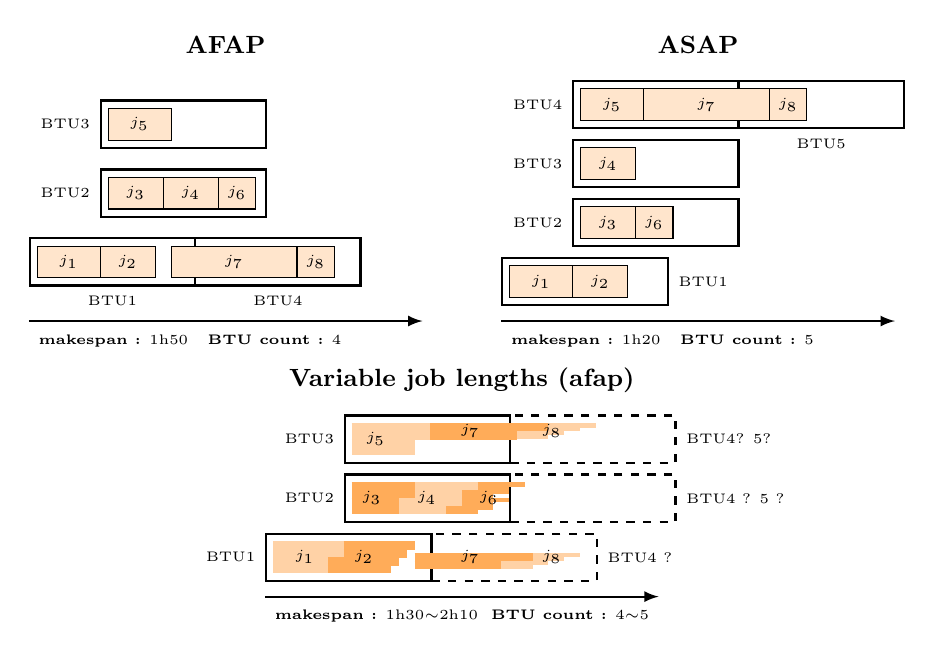
\begin{tikzpicture}[
desc/.style={
font=\small\bfseries,
},
job/.style={%
font=\tiny,
anchor=west,
fill=orange!20,
draw
},
inv/.style={%
font=\tiny,
anchor=west,
},
btu/.style={%
thick,
anchor=west,
draw,
minimum height=6mm,
minimum width=21mm,
},
capt/.style={
font=\tiny,
anchor=west,
}
]

%\draw[help lines](-6,-4)grid(6,4);

\begin{scope}[shift={(-5.5,0.5)}]
%Afap
\node[desc]at(2.5,3){AFAP};
\draw[-{latex},thick](0,-0.5)--(5,-0.5);
\node[btu,label={[font=\tiny]south:BTU1}]at(0,0.25){};
\node[btu,label={[font=\tiny]south:BTU4}]at(2.1,0.25){};
\node[job,minimum width=8mm]at(0.1,0.25){$j_1$};
\node[job,minimum width=7mm]at(0.9,0.25){$j_2$};
\node[job,minimum width=16mm]at(1.8,0.25){$j_7$};
\node[job,minimum width=4mm]at(3.4,0.25){$j_8$};

\node[btu,label={[font=\tiny]west:BTU2}]at(0.9,1.125){};
\node[job,minimum width=7mm]at(1,1.125){$j_3$};
\node[job,minimum width=7mm]at(1.7,1.125){$j_4$};
\node[job,minimum width=4mm]at(2.4,1.125){$j_6$};

\node[btu,label={[font=\tiny]west:BTU3}]at(0.9,2){};
\node[job,minimum width=8mm]at(1,2){$j_5$};

\node[capt]at(0,-0.75){\textbf{makespan :} 1h50~~~\textbf{BTU count :} 4};

\end{scope}

\begin{scope}[shift={(0.5,0)}]
%Asap
\node[desc]at(2.5,3.5){ASAP};
\draw[-{latex},thick](0,0)--(5,0);
\node[btu,label={[font=\tiny]east:BTU1}]at(0,0.5){};
\node[job,minimum width=8mm]at(0.1,0.5){$j_1$};
\node[job,minimum width=7mm]at(0.9,0.5){$j_2$};

\node[btu,label={[font=\tiny]west:BTU2}]at(0.9,1.25){};
\node[job,minimum width=7mm]at(1,1.25){$j_3$};
\node[job,minimum width=4mm]at(1.7,1.25){$j_6$};

\node[btu,label={[font=\tiny]west:BTU3}]at(0.9,2){};
\node[job,minimum width=7mm]at(1,2){$j_4$};

\node[btu,label={[font=\tiny]west:BTU4}]at(0.9,2.75){};
\node[btu,label={[font=\tiny]south:BTU5}]at(3,2.75){};
\node[job,minimum width=8mm]at(1,2.75){$j_5$};
\node[job,minimum width=16mm]at(1.8,2.75){$j_7$};
\node[job,minimum width=4mm]at(3.4,2.75){$j_8$};

\node[capt]at(0,-0.25){\textbf{makespan :} 1h20~~~\textbf{BTU count :} 5};
\end{scope}

\begin{scope}[shift={(-2.5,-3.5)}]
\node[desc]at(2.5,2.75){Variable job lengths (afap)};
\draw[-{latex},thick](0,-0)--(5,-0);
\node[btu,label={[font=\tiny]west:BTU1}]at(0,0.5){};
\node[btu,dashed,label={[font=\tiny]east:BTU4 ?}]at(2.1,0.5){};
\draw[color=orange!35,line width=2.1mm](0.1,0.6)--(1,0.6);
\draw[color=orange!35,line width=2.1mm](0.1,0.4)--(0.8,0.4);
\node[inv,minimum width=8mm]at(0.1,0.5){$j_1$};
\draw[color=orange!65,line width=1.1mm](1,0.65)--(1.9,0.65);
\draw[color=orange!65,line width=1.1mm](1,0.55)--(1.8,0.55);
\draw[color=orange!65,line width=1.1mm](0.8,0.45)--(1.7,0.45);
\draw[color=orange!65,line width=1.1mm](0.8,0.35)--(1.6,0.35);
\node[inv,minimum width=7mm]at(0.9,0.5){$j_2$};
\draw[color=orange!65,line width=1.1mm](1.9,0.50)--(3.4,0.50);
\draw[color=orange!65,line width=1.1mm](1.9,0.40)--(3,0.40);
\node[inv,minimum width=16mm]at(1.8,0.5){$j_7$};
\draw[color=orange!35,line width=0.55mm](3.4,0.525)--(4,0.525);
\draw[color=orange!35,line width=0.55mm](3.4,0.475)--(3.8,0.475);
\draw[color=orange!35,line width=0.55mm](3,0.425)--(3.6,0.425);
\draw[color=orange!35,line width=0.55mm](3,0.375)--(3.4,0.375);
\node[inv,minimum width=4mm]at(3.4,0.5){$j_8$};

\node[btu,label={[font=\tiny]west:BTU2}]at(1,1.25){};
\node[btu,dashed,label={[font=\tiny]east:BTU4 ? 5 ?}]at(3.1,1.25){};
\draw[color=orange!65,line width=2.1mm](1.1,1.35)--(1.9,1.35);
\draw[color=orange!65,line width=2.1mm](1.1,1.15)--(1.7,1.15);
\node[inv,minimum width=7mm]at(1,1.25){$j_3$};
\draw[color=orange!35,line width=1.1mm](1.9,1.4)--(2.7,1.4);
\draw[color=orange!35,line width=1.1mm](1.9,1.3)--(2.5,1.3);
\draw[color=orange!35,line width=1.1mm](1.7,1.2)--(2.5,1.2);
\draw[color=orange!35,line width=1.1mm](1.7,1.1)--(2.3,1.1);
\node[inv,minimum width=7mm]at(1.7,1.25){$j_4$};
\draw[color=orange!65,line width=0.55mm](2.7,1.425)--(3.3,1.425);
\draw[color=orange!65,line width=0.55mm](2.7,1.375)--(3.1,1.375);
\draw[color=orange!65,line width=0.55mm](2.5,1.325)--(3.1,1.325);
\draw[color=orange!65,line width=0.55mm](2.5,1.275)--(2.9,1.275);
\draw[color=orange!65,line width=0.55mm](2.5,1.225)--(3.1,1.225);
\draw[color=orange!65,line width=0.55mm](2.5,1.175)--(2.9,1.175);
\draw[color=orange!65,line width=0.55mm](2.3,1.125)--(2.9,1.125);
\draw[color=orange!65,line width=0.55mm](2.3,1.075)--(2.7,1.075);
\node[inv,minimum width=4mm]at(2.6,1.25){$j_6$};

\node[btu,label={[font=\tiny]west:BTU3}]at(1,2){};
\node[btu,dashed,label={[font=\tiny]east:BTU4? 5?}]at(3.1,2){};
\draw[color=orange!35,line width=2.1mm](1.1,2.1)--(2.1,2.1);
\draw[color=orange!35,line width=2.1mm](1.1,1.9)--(1.9,1.9);
\node[inv,minimum width=8mm]at(1,2){$j_5$};
\draw[color=orange!65,line width=1.1mm](2.1,2.15)--(3.6,2.15);
\draw[color=orange!65,line width=1.1mm](2.1,2.05)--(3.2,2.05);
\node[inv,minimum width=16mm]at(1.8,2.1){$j_7$};
\draw[color=orange!35,line width=0.55mm](3.6,2.175)--(4.2,2.175);
\draw[color=orange!35,line width=0.55mm](3.6,2.125)--(4,2.125);
\draw[color=orange!35,line width=0.55mm](3.2,2.075)--(3.8,2.075);
\draw[color=orange!35,line width=0.55mm](3.2,2.025)--(3.6,2.025);
\node[inv,minimum width=4mm]at(3.4,2.1){$j_8$};
\textasciitilde
\node[capt]at(0,-0.25){\textbf{makespan :} 1h30$\sim$2h10~~\textbf{BTU count :} 4$\sim$5};
\end{scope}


\end{tikzpicture}
